\section{RISE}
Like LIME, RISE is a block box method and works on manipulation of the input images. Instead of using superpixels, RISE generates masks that are then applied to the input images


\begin{figure}[H]
    \centering
    \begin{subfigure}[t]{.30\textwidth}
        \centering
        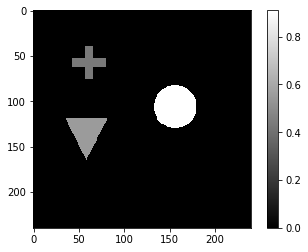
\includegraphics[width=\linewidth]{chapters/02_methods/images/rise/rise_original.png}
        \caption{}
    \end{subfigure}\hfill%
    \begin{subfigure}[t]{.30\textwidth}
        \centering
        \includegraphics[width=\linewidth]{chapters/02_methods/images/rise/rise_mask0.png}
        \caption{}
    \end{subfigure}\hfill%
    \begin{subfigure}[t]{.30\textwidth}
        \centering
        \includegraphics[width=\linewidth]{chapters/02_methods/images/rise/rise_mask0.png}
        \caption{}
    \end{subfigure}
    \caption{Superpixels generated for an input image. Superpixels are the features LIME analyzes to detect if they are relevant for the classification.\cite{limeoreilly}}
    \label{lime_superpixel}
\end{figure}

\begin{figure}[H]
    \centering
    \begin{subfigure}[t]{.35\textwidth}
        \centering
        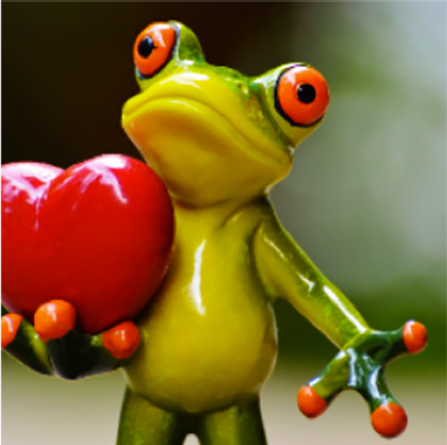
\includegraphics[width=\linewidth]{chapters/02_methods/images/frog1.png}
        \caption{Original image}
    \end{subfigure}\hspace{1.5cm}%
    \begin{subfigure}[t]{.35\textwidth}
        \centering
        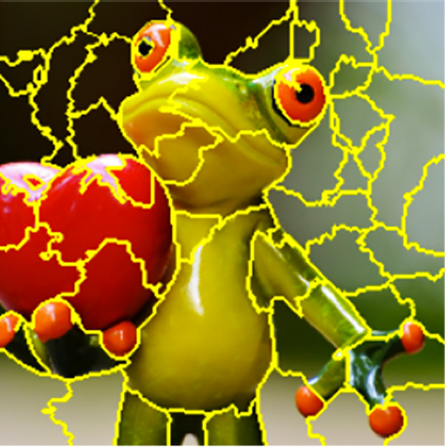
\includegraphics[width=\linewidth]{chapters/02_methods/images/frog2.png}
        \caption{Original image overlaid with superpixel boundaries}
    \end{subfigure}
    \caption{Superpixels generated for an input image. Superpixels are the features LIME analyzes to detect if they are relevant for the classification.\cite{limeoreilly}}
    \label{lime_superpixel}
\end{figure}



Figure \ref{TODO}

Original implementation written for PyTorch.

TODO: show masks
TODO: explain the matrix multiplication

\begin{figure}[H]
\centering
\caption{Image from original paper explaining some classes}
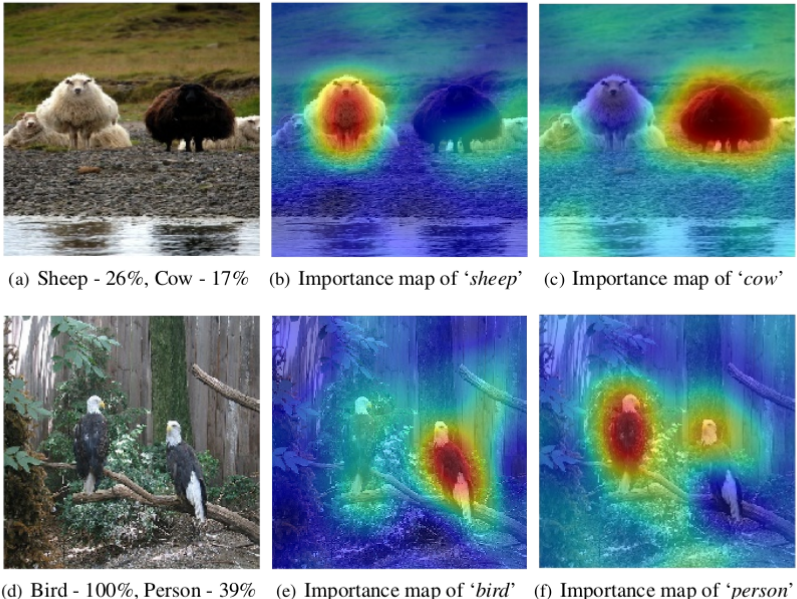
\includegraphics[width=12cm]{chapters/02_methods/images/rise.png}
\end{figure}


* [ ] doc: RISE: explain heatmap, why is it there? => gaus, upsampling
